\section{Evaluation}
In this section, we show the feasibility of the approach of using declarative
analysis for multilingual program, and the effectiveness of its
implementation. More specifically, we set three research questions as follow:

RQ1) Feasibility: Is it possible to implement a working static analyzer for multilingual program in declarative style?

RQ2) Performance: How is the speed and precision of implemented analyzer, compared to the state-of-the-art analyzer?

RQ3) Usefulness: How practical is the implemented analyzer?

To answer RQ1, we ran our implemented analyzer to NativeFlowBench, which is a
small set of benchmarks manually crafted by authors of JN-SAF[2], with the
purpose of testing dataflow analyzer for JNI programs. It consists of 23
android applications featuring various interactions between C++ and Java, some
of which contain a malicious code pattern that tries leak sensitive user data.
To answer RQ2, we ran our analyzer to 42 real-world android applications
collected from F-Droid[9], a repository for open-source android application. These
42 apps are selected by searching for apps with JNI, and among them, selecting those
that we could successfully compile. We compared our analyzer with
state-of-the-art[3] JNI analyzer, and confirmed that our analyzer outperforms
in terms of scalability and precision. To answer RQ3, we implemented various
kinds of bug checkers, illustrated in previous researches[1][3], on top of our
analyzer. We ran our bug checker on the 42 applications of F-Droid mentioned
above, and discovered \inred{??} bugs, including \inred{??} newly found bugs.


\subsection{RQ1: Feasibility}
\begin{figure*}[t]
  \centering
  \vspace{2mm}
  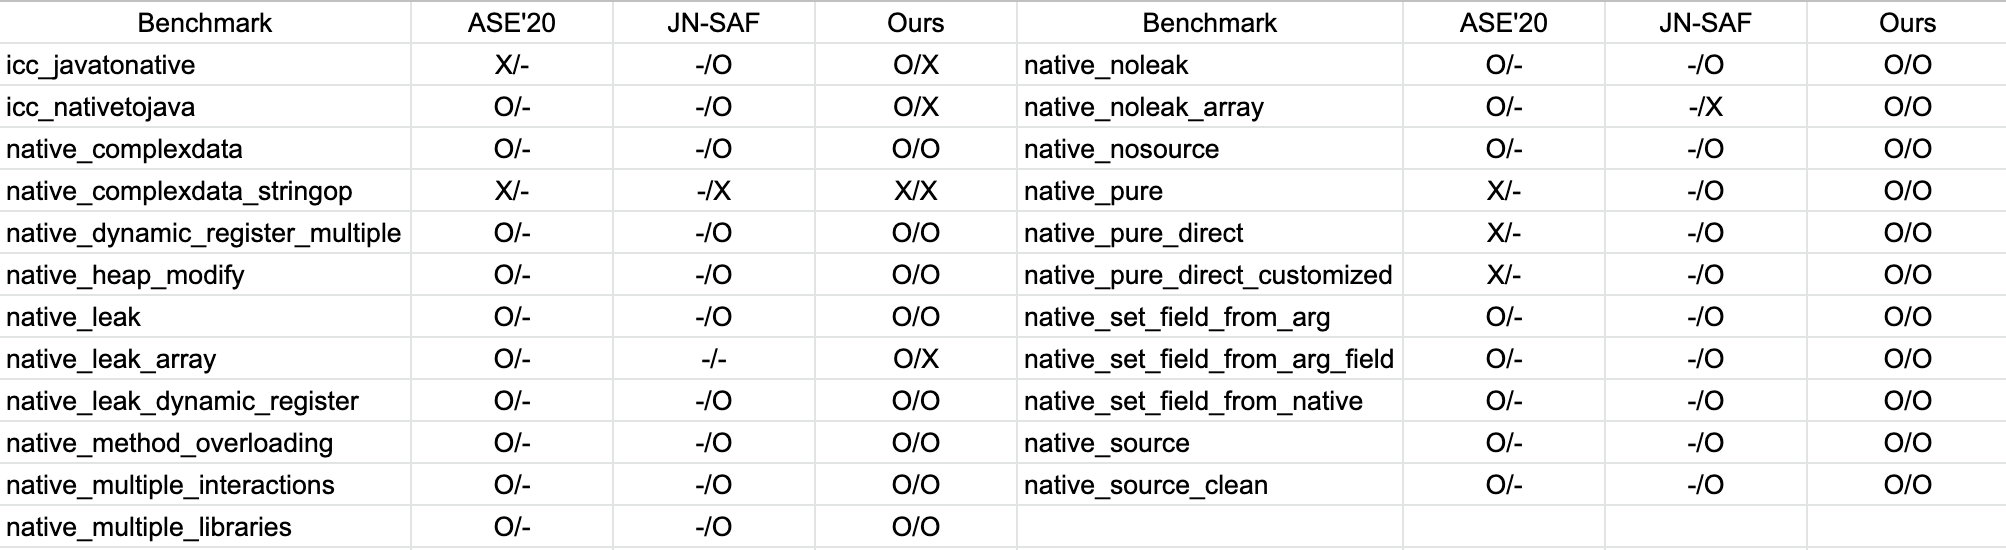
\includegraphics[width=\textwidth]{img/table1}
  \vspace*{-1.5em}
  \caption{The analysis result of NativeFlowBench}
  \label{fig:table1}
\vspace*{-.5em}
\end{figure*}

Table~\ref{fig:table1} shows the analysis result for 19 benchmarks in NativeFlowBench.  The
"Benchmark" columns denote the benchmark names, and "ASE'20", "JN-SAF", "Ours"
columns denote whether the analysis result for corresponding benchmark was
correct(O), incorrect(X), or not available(-) in terms of two criteria for each
of the implementation.  The left denotes precision result, where we call that
the analysis result is successful if every function call target (call(j->c),
call(c->j)) and field access target (field\_read(c->j), field\_write(c->j)) are
precisely determined. The right denotes dataflow result, where it's considered
correct if every data leak is reported correctly without false positives nor
false negatives. 

For the precision result, except for one benchmark, our analyzer could
correctly determine all targets for function calls and field access correctly,
and could successfully perform dataflow analysis to find all of the data leaks.
The only exception was native\_complexdata\_stringop, where string manipulation
functions such as strcpy or strcat from C++'s standard library were used to
create the string value that indicates the target method's name, and since the
inner-flow analysis could not properly handle these functions, analyzer could
not correctly determine the function call target. This is superior result to
the ASE'20, which could not precisely analyze the 4 additional benchmarks.

For the dataflow result, we compare the result with JN-SAF. There were 3 benchmarks
that our analyzer failed to detect leak. Two of them are related to inter component
communication(ICC), which is a android-specific feature and was out of scope for
our implementation. The other one was related to array. The data is stored in
array and read. Since our base analyzer could not model the data flow through
array, this kind of leak was not detected.

As a result, we could conclude that it is feasible to implement
static analysis in declarative style, in that it shows competable
analysis result for the given benchmark.


\subsection{RQ2: Performance}
\begin{figure*}[t]
  \centering
  \vspace{2mm}
  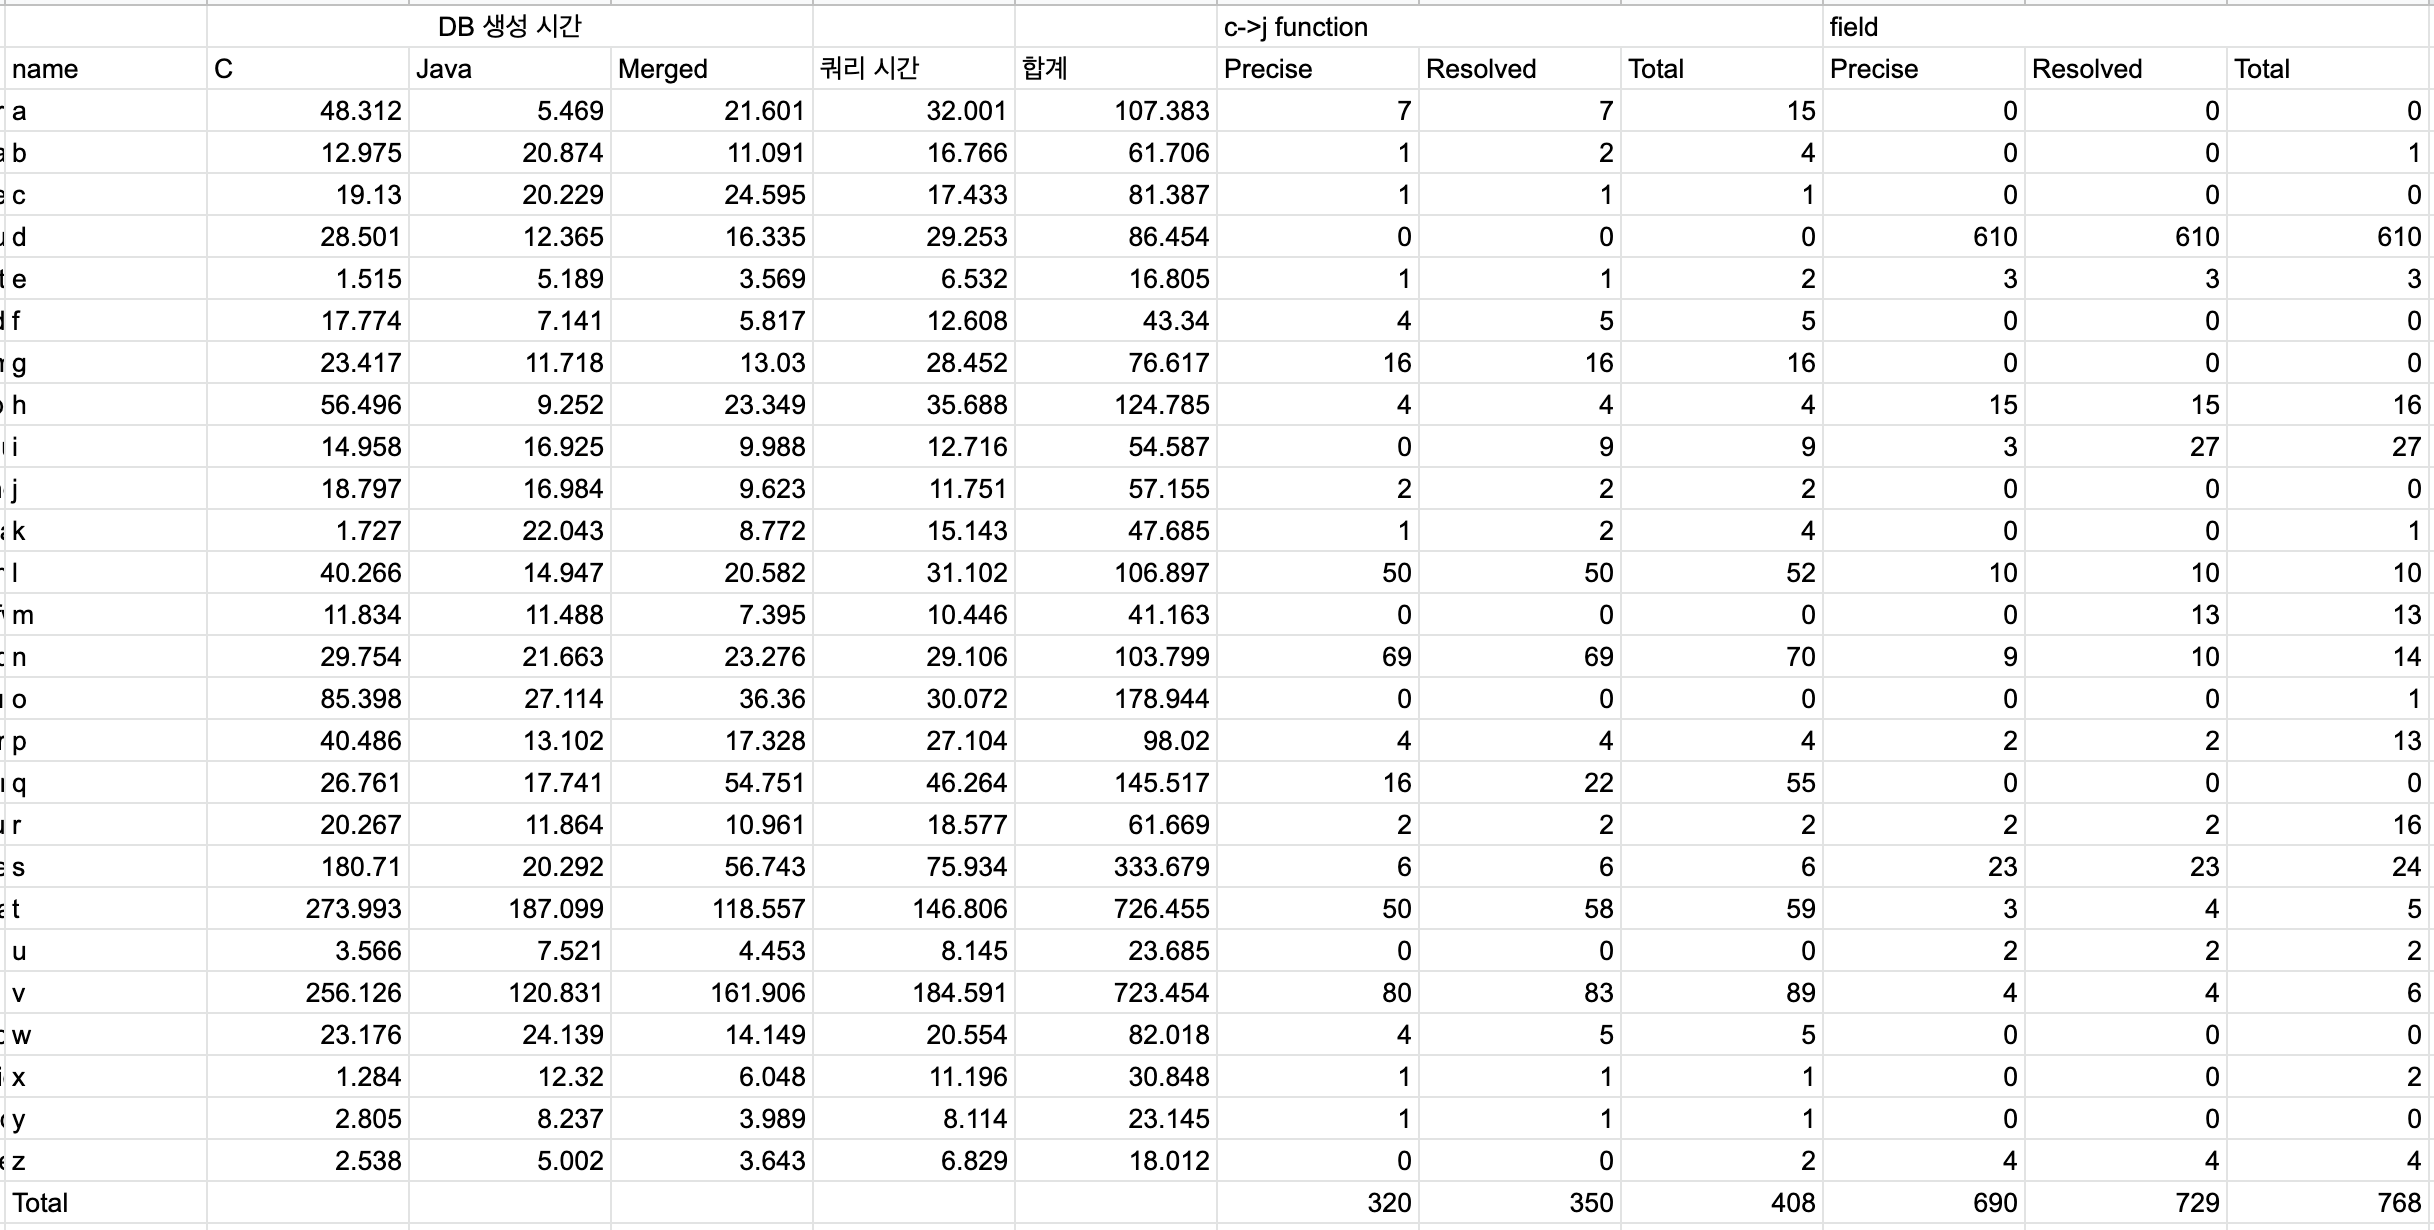
\includegraphics[width=\textwidth]{img/table2}
  \vspace*{-1.5em}
  \caption{The analysis result for F-Droid applications}
  \label{fig:table2}
\vspace*{-.5em}
\end{figure*}

Table~\ref{fig:table2} shows the analysis result for F-Droid applications. We summarize
result for 25 of 42 apps, which contains Java method or field access
from C. \inred{The full list of data is available at ???}.

The "time" column denotes the time for creating database and evaluating query.
The average time for creating DB was ??? seconds, and average time for
evaluating query was ???  seconds, making the average of total analysis time
??? seconds. 

\begin{figure}[t]
  \centering
  \vspace{2mm}
  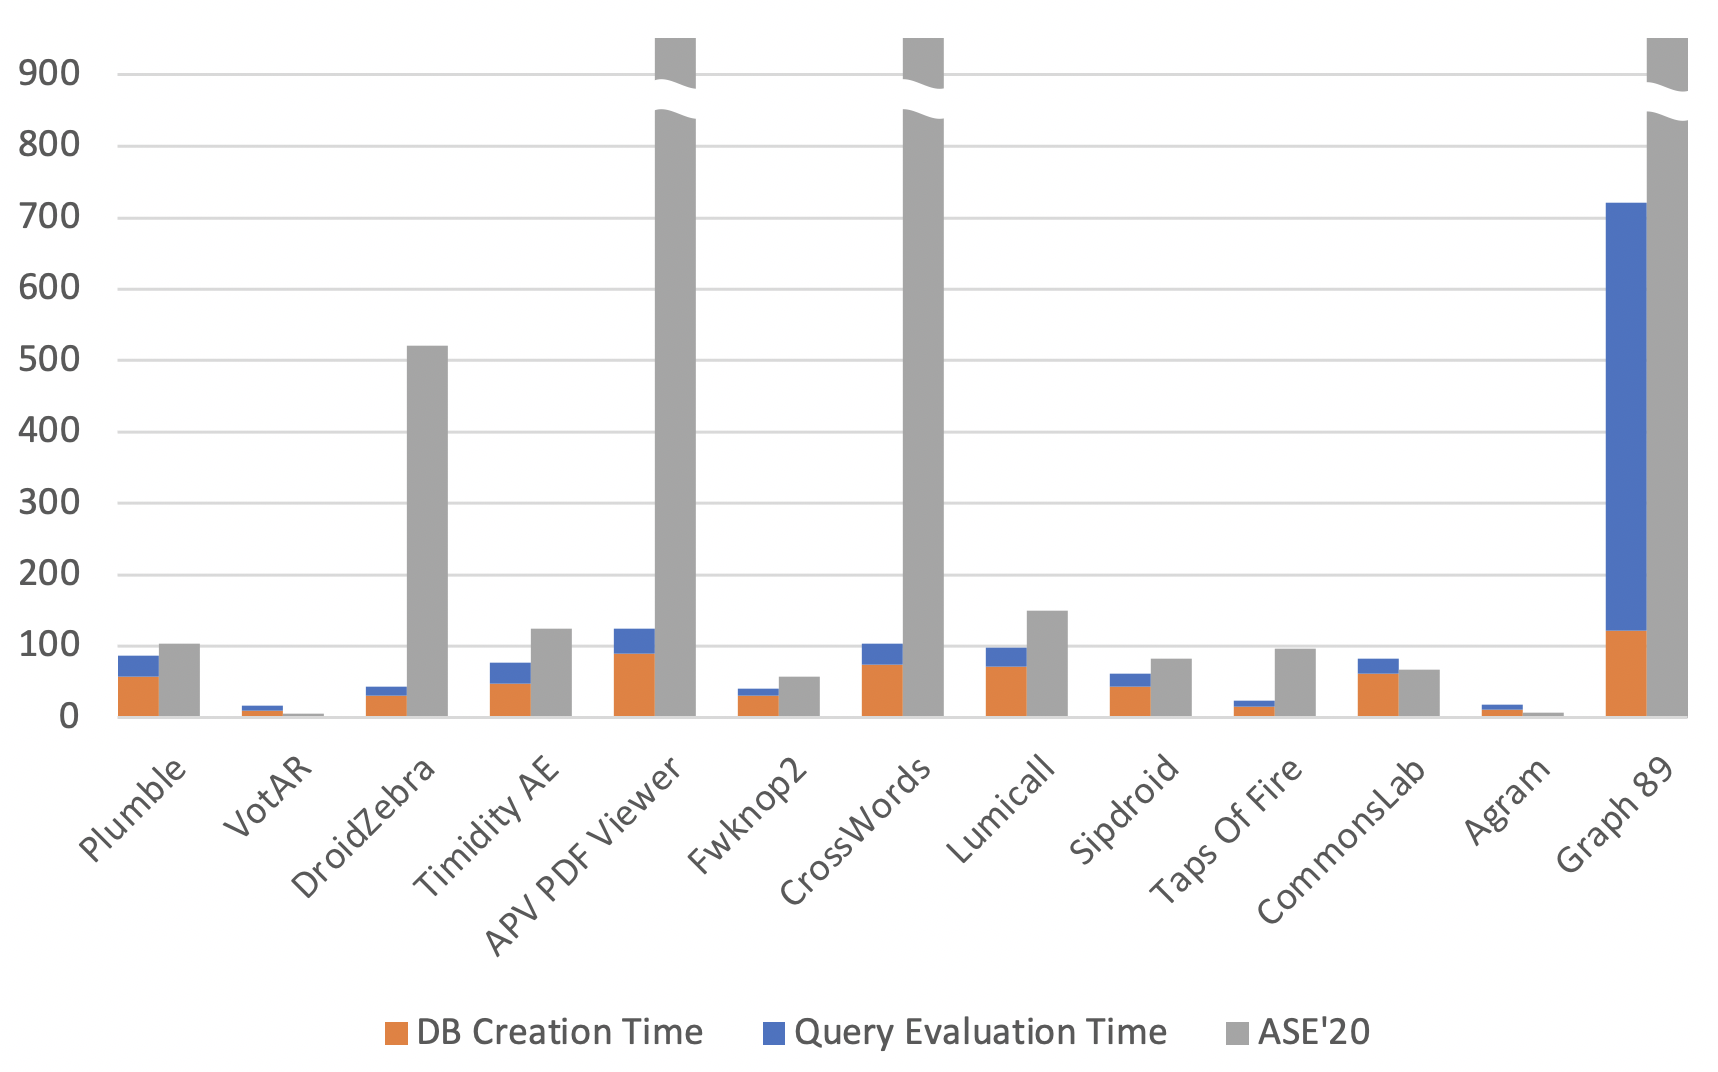
\includegraphics[width=0.5\textwidth]{img/graph}
  \vspace*{-1.5em}
  \caption{Speedup}
  \label{fig:graph}
\vspace*{-.5em}
\end{figure}

Among 25 apps, 13 of them were included in benchmark of ASE'20, and the
evaluation time with their tool is available.  Figure~\ref{fig:graph} shows the speed per
application, one by one.  The average speed up was x4. Note that time for
creating DB is done by comping source code, which is excluded from the calculated
time of ASE'20. This means that we also have to exclude the time for creating DB
from our calculated time, which makes the practical speed up become x14.

The "precision" columns denotes the precision of dispatching function call
target, and field access target.  "Precise" means exactly one target was found,
and resolved means at least one target was found. For the function call from C to Java,
\inred{???}\% of function calls were resolved, and \inred{???}\% of functions calls
were precisely resolved. For the field access, \inred{???}\% of field accesses (both
read and write) were resolved, and \inred{???}\% of field access were precisely resolved.
Compared to the precision result of the state-of-the-art analyzer, our implementation
showed higher precision.

The main reason that the analyzer failed to resolve some of the function calls
or field accesses is due to the lack of soundness of base-line CodeQL dataflow
analysis library.  Specifically, if function pointer is involved when calling C
function within C, CodeQL could not determine the exact call target, and some
data which is needed for determining the Java method call target is not
analyzed to be passed, resulting in failure to resolving Java method target.

In conclusion, considering that our analyzer could successfully analyze the
benchmark applications with higher precision in significantly shorter time
compared to the stat-of-the-art analyzer, we conclude that our implementation
has competitive performance.

\subsection{RQ3: Usefulness}
\begin{figure}[t]
  \centering
  \vspace{2mm}
  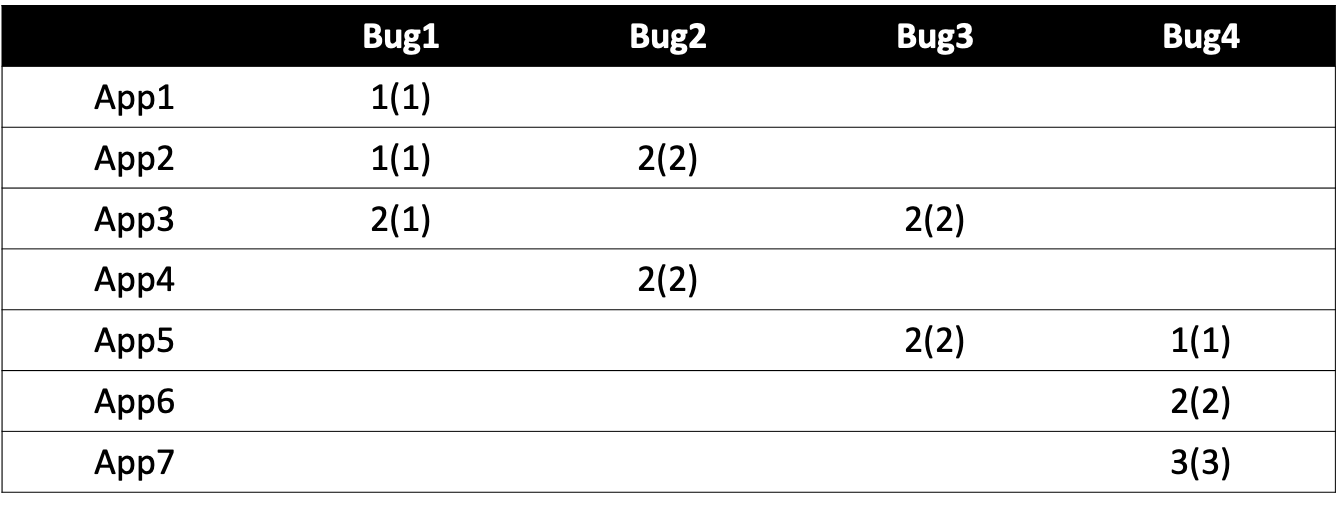
\includegraphics[width=0.5\textwidth]{img/table3}
  \vspace*{-1.5em}
  \caption{The list of bugs and security vulnerabilities checkers}
  \label{fig:table3}
\vspace*{-.5em}
\end{figure}

Table~\ref{fig:table3} shows the list of bugs and security vulnerabilities we could detect.
The first bug is the null dereference bug[1][9], which detects the dereference of
Java's null value in C, without proper nullity checking logic. Rest of three
bugs are related to mistake in using interaction, which are described in
previous research[2]. "Missing fun" denotes the case where C function is
missing even if it is called from java. "Type mismatch" denotes the case where
the declaration of native function in Java has different return type or
parameter type with its actual definition in C.  "Wrong signature" denotes the
case where "GetMethodID" uses wrong signature for the java method. The
number in each cell denotes the number of alarms, and the number in the
parenthesis denotes the number of false alarm, if any.

\begin{figure}[t]
  \centering
  \vspace{2mm}
  \begin{subfigure}[t]{0.5\textwidth}
    \begin{lstlisting}[style=cpp,xleftmargin=2.5em]
//EmulatorActivity.java
String tmp = null;
String folder = Util.GetInternalAppStorage(activity);

if (folder != null) {
  tmp = folder + "tmp";
  Util.CreateDirectory(tmp);
}

EmulatorActivity.nativeInitGraph89(..., tmp);

//wrappercommonjni.c
void Java_..._nativeInitGraph89(..., jstring tmp_dir) {
   (*env)->GetStringUTFChars(env, tmp_dir, 0);
   ...
}
    \end{lstlisting}
    \vspace*{-.5em}
    \caption{Null dereference}
    \label{fig:bug1}
  \end{subfigure}
  \begin{subfigure}[t]{0.5\textwidth}
    \begin{lstlisting}[style=cpp,xleftmargin=2.5em]
//JpegRedaction.java
package org.witness.obscuracam.photo.jpegredaction;

public class JpegRedaction {
  private native void redactRegions(...);
  ...
}

//JpegRedaction.cpp
void
Java_org_witness_securesmartcam_jpegredaction_ JpegRedaction_redactRegions(...) {
  ...
}
    \end{lstlisting}
    \vspace*{-.5em}
    \caption{Missing Fun}
    \label{fig:bug2}
  \end{subfigure}
  \begin{subfigure}[t]{0.5\textwidth}
    \begin{lstlisting}[style=cpp,xleftmargin=2.5em]
//MuPdfPage.java
private native static List<PageTextBox> search(...);

//mupdfdroidbridge.c
jobjectArray Java_..._search(...){
   ...
 }
    \end{lstlisting}
    \vspace*{-.5em}
    \caption{Type Mismatch}
    \label{fig:bug3}
  \end{subfigure}
  \begin{subfigure}[t]{0.5\textwidth}
    \begin{lstlisting}[style=cpp,xleftmargin=2.5em]
//PrBoomActivity.java
void OnMessage(String text);
void OnInfoMessage(String msg, int displayType);

//jni_doom.h
#define CB_CLASS_MSG_SIG  "(Ljava/lang/String;I)V"
#define CB_CLASS_INFMSG_SIG  "(Ljava/lang/String;I)V"

//jni_doom.c
mSendStr = (*env)->GetMethodID(env, jNativesCls, "OnMessage", CB_CLASS_MSG_SIG);

    \end{lstlisting}
    \vspace*{-.5em}
    \caption{Wrong Signature}
    \label{fig:bug3}
  \end{subfigure}
  \vspace*{-.5em}
  \caption{Real excerpt of examples of bugs}
  \label{fig:bugs}
\end{figure}

We demonstrate some interesting bugs we found in our benchmark with actual minified examples above
for each kind.

First example denotes null dereference bug. A null is stored in variable tmp, and
it is updated into non-null value under certain condition. However, tmp is passed
to a C function even if it is still null, and it is dereferenced there
without proper check.

Second example denotes a bug where C function is missing. The name for target C
function is decided with convention, and the java package's name is used
for deciding the name. It seems that package name is changed during development,
but the function name in the C source code was not changed respectively, resulting
in missing function bug.

In third example, the return type of the function is List, which is an object.
However, in C, the return type of the function is defined as "jarray", which
should be used for array, not object.

In the final example, it demonstrates the case where wrong signature is used
for dispatching java method from C, using "GetMethodID" function. An interesting
point is that, the signatures were defined in C macro, and the wrong signature
was the same as the next one.

We manually inspected the source code if the reported alarms are false positive
or not. No false positives were found for latter three kinds of bugs.  There
were some false positive for the first bug, the null dereference bug. The
reason for these false positives were mainly due to, again, imprecise
intra-language dataflow. For example, the analyzer could not handle the case
where a variable is reassigned to a non-null value in a different branch or a
different function, resulting in giving the false positive that null value can
be dereferenced.

In summary, we can conclude that our analyzer is practical and useful enough,
in that we could find previously unknown bugs/security vulnerabilities using
our analyzer.
